\documentclass{article}
% Packages
\usepackage{algorithm}
\usepackage{algorithmic}
\usepackage{hyperref}
\usepackage{geometry}
\usepackage{graphicx}
\usepackage{titlesec}
\usepackage{amsmath}

% Customize the title format
\newgeometry{vmargin={30mm}, hmargin={50mm,50mm}}
% Title
\title{ Technical Report --- EGB242 Assignment 1}
\author{Matiu Kaufusi\\N10541977}



\begin{document}

% Cover page
\begin{titlepage}
    \begin{center}
        \begin{tabular}{c@{\hskip 5cm}l}
            \multicolumn{1}{r}{%
                \begin{minipage}{.6\textwidth}
                    \raggedleft
                    \LARGE \textbf{Queensland University}\\
                    \LARGE \textbf{of Technology}
                \end{minipage}
            } & \raisebox{-0.6\height}{
\includegraphics[width=2cm]{logo.jpg}} % also works with logo.pdf
        \end{tabular}
    \end{center}

    \centering
    \vfill
    {\bfseries\Large
        EGB242 Assignment 1 -- Report\\
        2023 Semester 1\\
        \vskip2cm
        Matiu Kaufusi\\
        \vskip1cm
        Bachelor of Engineering (Honours)\\
        Computer and Software Systems Major\\
    }
    \vfill

    \vfill
    \vfill
\end{titlepage}

\newpage
% Table of contents
\tableofcontents
\newpage
‌\section{Introduction}
At BASA (Brisbane's premiere space angency) the task of finalising the design of the communication system components was presented. The design components were microphone, radio transmitter, radio receiver, analog-to-digital converter.
\par
This report will detail the design process undertaken. Removing the noise from the newly installed microphone comes first. Modulating the signal onto a carrier frequency for radio transmission, then demodulation for the radio receiver is next. Lastly, converting the audio from an analog signal to a digital signal in order for distribute the audio to astronaut headphones and other ship systems completes the design.
\section{Periodic Noise Removal}
The microphone is a key component in the communication system. The microphone is used to capture the audio from the mission control room and send it to the astronaut headphones. After inspection on the audio waveform produced by the microphone, it was found that the microphone was producing a periodic noise. The cause for the noise is still undetermined but certain factors like: the microphone being located near a source of electromagnetic interferance, certian enviornmental conditions, and faulty microphone hardware are all possible causes.
\subsection{Noise Removal Process}
To remove the noise, the additive process must be reversed. The additive process has the audio signal $a(t)$ added to the noise signal $n(t)$ to produce the output signal $o(t)$. To reverse this process, the noise signal $n(t)$ must be subtracted from the output signal $o(t)$ to produce the audio signal $a(t)$. Thanks to a fellow BASA engineer the model for the noise signal was found to be the following:
\begin{equation}
    n(t) =
    \left\{
        \begin{array}{lr}
            5e^{4(t-1)}\;\;\;\; 0 \leq t < 1\\
            -3t + 8\;\;\;\; 1 \leq t < 2
        \end{array}
    \right\}
    \end{equation}
To start with the audio was replayed to confirm the periodic noise. The periodic noise confirmed to be present, and was confirmed to have clipping. The clipping was confirmed by the slight increase in loudness. The audio also now had high frequency blips at the even integers of the $o(t)$ signal.
\subsection{Complex Fourier Series}
The noise removal process used in this scenario will utilise the complex Fourier series. The complex Fourier series is a series of complex exponentials that can be used to represent any periodic signal. The complex Fourier series is defined as:
\begin{equation}
    s(t) = \sum_{n=-\infty}^{\infty} c_n e^{j2 \pi nf_{0}t}
\end{equation}
Where $c_n$ is the complex coefficient of the $n^{th}$ term, $f_{0}$ is the fundamental frequency, and $j$ is the imaginary unit. To calculate the complex coefficent of the $n^{th}$ term, the following equation is used:
\begin{equation}
    c_n = \frac{1}{T} \int_{t_{0}}^{t_{0}+T} s(t) e^{-j2 \pi nf_{0}t} dt
\end{equation}
Where $T$ is the period of the signal, and $t_{0}$ is the starting time of the signal. Calculations for the complex Fourier coefficent $c_{0}$ and its complex Fourier Series can be found in section \ref{sec:Fourier} of the appendix. Using $-5 \leq n \leq 5$ (i.e., 5 harmonics) to generate an approximation of of the noise signal \ref{sec: nApprox}, we can de-noise the audio signal \ref{sec: Audio} by reversing the additive process. The final output is a clean audio signal with high frequency blips even integer time intervals \ref{sec: CleanAudio}. It was also tested using $-50 \leq n \leq 50$ (i.e., 50 harmonics) to generate an approximation of of the noise signal. This resulted in more crisp and clear voice audio but did not reduce the high frequency blips at the even integer time intervals.

\section{Modulation and Demodulation}
\subsection{Modulation}
Modulation is the process of "moving" a time-domain signal to a frequency-domain signal. The reason for modulation is to allow the possibility of audio transmission as a radio signal by shifting the signal to a higher band of frequencies. The modulation proccess used is known as Amplitude Modulation (AM) and is characterized by the fact that the amplitude A of the carrier signal is varied in proportion to the audio signal. Using the MATLAB \textit{channel.p} function simulating the transmission of a signal \textit{input} between the ground station and the orbiter can be observed by entering the following command:
$$output = channel(sid,\;input)$$
Through the use of this command the channel can be listend to by passing a vector of zeros though the channel function like so:
\begin{align}
\raggedright
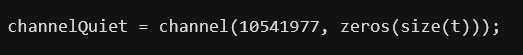
\includegraphics[width=\textwidth,height=\textheight,keepaspectratio]{channelQuiet.png}
\end{align}
The \textit{channelQuiet} time domain \ref{sec: ChannelTime} and frequency domain plots show the channels attributes. In terms of frequency bandwidth, it is usually needed to be twice as large as the largest frequency component in the original audio signal. Observing \ref{sec: CleanAudioFreq} the largest frequency component can be said to be around 4kHz. Using the frequency domain plot \ref{sec: ChannelFreq} to find an empty bandwidth large enough to accomadate 4kHz can be seen in the ranges fof 45,000 Hz - 75,000 Hz. The gives us a center frequency of 60 kHz. This carrier frequency provides enough bandwidth to cover the voice and provides a clear and distinct aduio output. Modulating the clean audio signal is done by multiplying the carrier signal by the audio signal, examplified in this code snippet:
\begin{align}
\raggedright
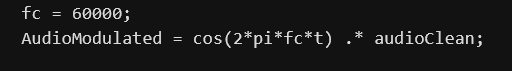
\includegraphics[width=\textwidth,height=\textheight,keepaspectratio]{modulation.png}
\end{align}
\subsection{Demodulation}
Demodulation is the process of "moving" a frequency-domain signal to a time-domain signal. The reason for demodulation is to extract the original information from the modulated signal. Amplitude modulation (AM) is able to neatly demodulated by utilising the cosine trigonometric identity:
\begin{align}
\cos A\times \cos B= \frac{1}{2}\times\left(\cos(A-B)+\cos(A+B)\right)
\end{align}
This equates to the final expression being:
\begin{align}
    AudioDeModulated = \frac{1}{2}  \times audioClean \label{eq5}\\
    +\\
    \raggedright
    \frac{1}{2} \times audioClean \times \cos(4*\pi*f_{c}*t) \label{eq6}
\end{align}
This leaves us with the two components $0.5 \times audioClean$ which is the original audio with half of its amplitude and $\frac{1}{2}  \times audioClean \times \cos(4*\pi*f_{c}*t)$ which is the modulated audio with a carrier frequency of $2f_{c}$. This can be  observed in the demodulated audio signal plot \ref{sec: DemodAudio} where there are excess magnitude spikes on both extremes of the plot (\ref{eq6}) and a concentration of magnitude spikes centred around 0Hz(\ref{eq5}).
\section{Analog-to-Digital Conversion}
The audio signal has now be cleaned of its noise, modulated through AM, and demodulated by reversing the modulation process. The demodulated audio now allows the astrounauts' to listen to the audio sent from mission control room through analogous means. The headphones and speakers in the ship, however, are of digital type which implies the signal must be converted. Signal digitisation can be done through through a sampling and quantisation process.
\subsection{Sampling}
Sampling is the process of converting a continous-time signal into a discrete-time signal. Simply, it is the process of measuring the amplitude of a signal at regular time intervals and representing those values as a sequence of numbers. Sampling can easily be done by utilising the \textit{resample} function in MATLAB. The \textit{resample} function takes in 3 parameters: $X$, $P$, and $Q$. $X$ is the signal to be sampled, $P$ is the upsampling integral factor, and $Q$ is the decimating sampling factor. Choosing an upsampling factor that is too low (or there is no bandlimit), will result in reconstruction exhibiting imperfections known as aliasing. Aliasing is an effect that causes different signals to become indistinguishable (or aliases of one another) resulting in a robotic sounding output. Choosing an upsampling factor that is too high can lead to an increased data size, and increased computational time. Using the Nyquist–Shannon sampling theorem we can ascertain an upsampling frequency that is optimal for minimal aliasing and computational load. The Nyquist–Shannon sampling theorem states that a signal can be perfectly reconstructed from its samples if the sampling frequency is at least twice the highest frequency component of the signal. The Nyquist–Shannon sampling theorem can be expressed as:
$$X < \frac{f_{s}}{2}$$
$$X < \frac{192\;kHz}{2}$$
$$X < 96\;kHz$$
From the most common valid sampling rates, 48kHz is the closest to 96kHz. Therefore, the upsampling factor is set to 48kHz. The decimating sampling factor is set to 192kHz. The following code snippet shows how the sampling process is done in MATLAB:
\begin{align}
\raggedright
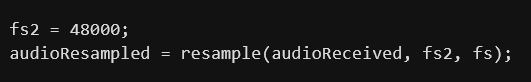
\includegraphics[width=\textwidth,height=\textheight,keepaspectratio]{resampled.png}
\end{align}
\subsection{Quantisation}
From the discrete-time signal generated from resampling, quantization replaces each real number with an approximation from a finite set of discrete values. Uniform quantizers can be categorised to be one of two types: \textit{mid-riser} (MR) and \textit{mid-tread} (MT). The \textit{mid-riser} uniform quantizer gets its name by having a rising section of its staircase centred at the origin. The \textit{mid-tread} uniform quantizer gets its name by having the flat section of the staircase centred at the origin. It is important to note that the \textit{mid-tread} quantizer is not centred about the y axis and therefore has $\pm1$ steps in its staircase compared to a \textit{mid-riser} of the same bit-level. Usually the additional step (even) is pushed to the negative side of the graph. Quantization levels refer to the step size between adjacent quantization levels in the MT and MR quantizers thus lowering quantize error. By increasing the number of steps one can increase the quality of the output. The step size used in this scenario is $16$ which is equal to $4\;bits$. The MATLAB code for this implementation is the following:
\begin{align}
\raggedright
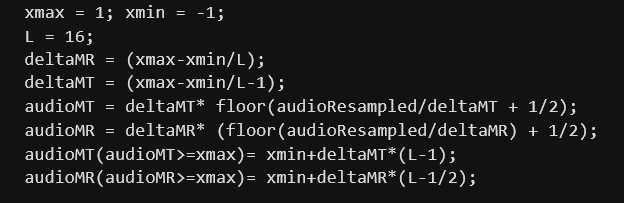
\includegraphics[width=\textwidth,height=\textheight,keepaspectratio]{N16.png} \label{Quantization: 16 levels}
\end{align}
This results in the mid-riser plot \ref{sec: N16MR}, and the mid-tread plot \ref{sec: N16MT}. After listening to both quantized audio and observing the plot, mid-tread is concluded to be the better choice.
\subsubsection{Quantization: 2, 4, 8, 32 levels}
For further analysis, the quantization levels 2, 4, 8, and 32 will be completed. Using the same formulae from \ref{Quantization: 16 levels}, the plots \ref{sec: VaryingLevels} can be generated for each corresponding quantization levels. Listening to the audio and observing the plots reveal MR to be an insufficent quantisation type for the given context. The audio is extremely amplified, causing clipping and distortion. MT at lower quantization levels is also not suitable for the given context. Observing the MT graphs reveals man inverse relationship between quantization noise and quantization levels, confirming the previous conclusion. The audio produced from 16 quantization levels and 32 quantization levels arent very different. This makes the choice of using 16 quantization levels the most plausible to lower computational load without sacrificing quality.






\section{Reflection}
In this assignment the key learning objectives are observed to be understanding the intricate concepts in signal analysis and communication systems. Beginning with the issue of periodic noise in an audio signal, modelling the noise as a complex fourier series then reversing the additive noise was done. Next was addressing the issue of modulatioin and demodulation of the cleaned audio signal, allowing the audio signal to be transmitted as an audio waveform and sent from ground station to spaceship.Choosing an appropriate carrier frequency was done by observing empty frequency bands, with enoguh bandwidth to contain the signal. Utilizing the Amplitude Modulation type by varying the carrier signal proportionally to the audio signal, efficient modulation and demodulation was achieved. Transmission of radio signals was able to be simulated Using the \textit{channel} MATLAB function provided. Using the output of this function, through quantization and sampling an analog to digital converter was produced to finally produce the audio signal in a digital format.
\bigbreak
Throughout the development of this assignment, valuable insights into the practical use and implementation of communication systems and signal processing techniques were. By far the most important lesson learned is how specific parameter choices affect the output greatly, such as the number of harmonics for the Fourier series approximation or the choice of carrier frequency for modulation. Changing these values greatly effected the output of each iterative design process, misdesign in any of these crucial steps would effect the rest of the remaining outputs to compute.Additionally, experimenting with different sampling rates and quantization levels provided more insight into aliasing and emphasized the trade-off between signal quality and resource constraints. If given the opportunity to approach this assignment again, I would explore alternative noise reduction techniques to rid my audio of the high frequency blips at times 2s, 4s, 6s, 8s, 10s. I would then compare their effectiveness in the context of the given problem. Investigation of different modulation schemes is also on the list of options i would like to explore the solution for. Lastly, i would like to look into quantization error techniques as the AM method used in this assignment did not produce the crisp audio i would've liked to hear.



\pagebreak
\section{References}


\pagebreak
\appendix
\section{Appendix}
\subsection{Fourier Coefficients and Series}
\label{sec:Fourier}
This is the first
\subsection{Noise approximation}
\label{sec: nApprox}
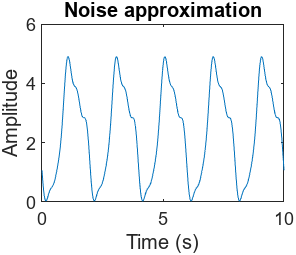
\includegraphics{nApprox.png}
\subsection{Audio with Noise}
\label{sec: Audio}
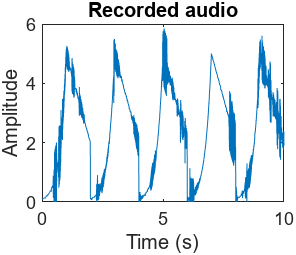
\includegraphics{AudioOutput.png}
\subsection{Clean Audio}
\label{sec: CleanAudio}
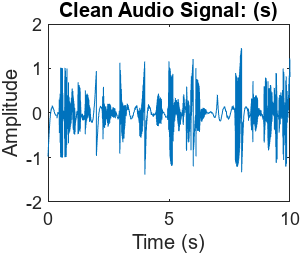
\includegraphics{CleanAudio.png}
\subsection{Clean Audio Frequency}
\label{sec: CleanAudioFreq}
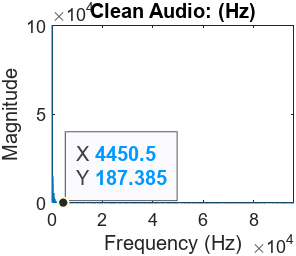
\includegraphics{audioCleanFreq.png}
\subsection{Channel Pre Transmission Time}
\label{sec: ChannelTime}
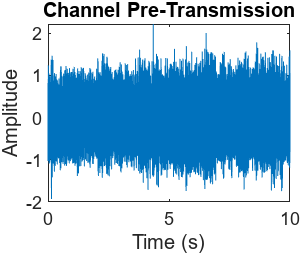
\includegraphics{channelQuietTimeDomain.png}
\subsection{Channel Pre Transmission Freq}
\label{sec: ChannelFreq}
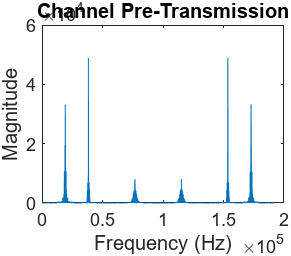
\includegraphics{channelQuietFreqDomain.png}
\subsection{Modulated Audio}
\label{sec: ModAudio}
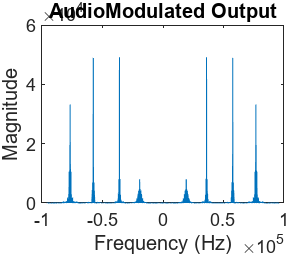
\includegraphics{modulated.png}
\subsection{Demodulated Audio}
\label{sec: DemodAudio}
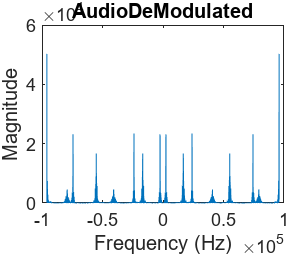
\includegraphics{demodulated.png}
\subsection{N16 Mid-Riser Audio}
\label{sec: N16MR}
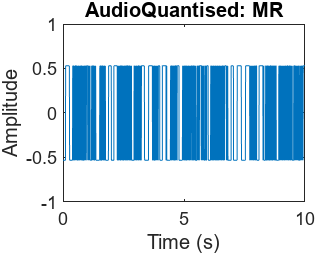
\includegraphics{N16MR.png}
\subsection{N16 Mid-Tread Audio}
\label{sec: N16MT}
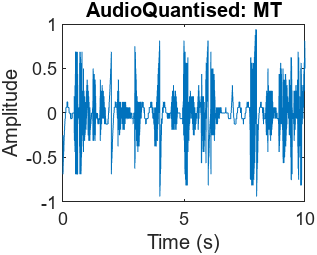
\includegraphics{N16MT.png}
\subsection{QuantizationAnalysis}
\label{sec: VaryingLevels}
\begin{figure}[!htb]
    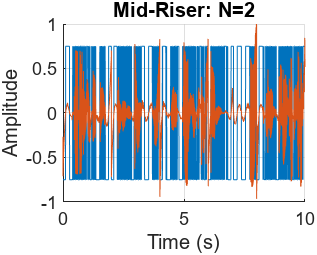
\includegraphics[width=.24\textwidth]{N2MR.png}\hfill
    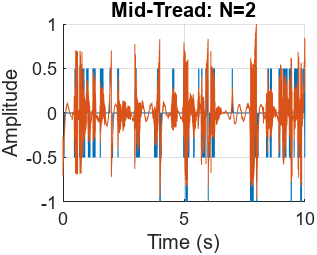
\includegraphics[width=.24\textwidth]{N2MT.png}\hfill
    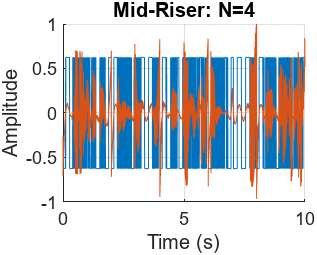
\includegraphics[width=.24\textwidth]{N4MR.png}\hfill
    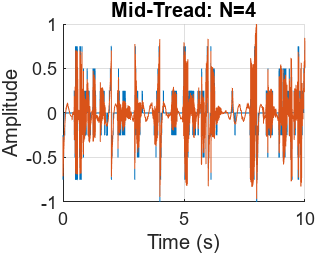
\includegraphics[width=.24\textwidth]{N4MT.png}\hfill
    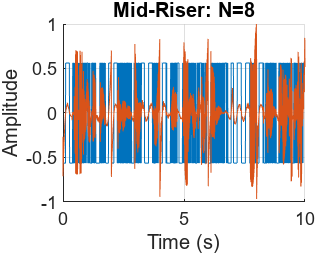
\includegraphics[width=.24\textwidth]{N8MR.png}\hfill
    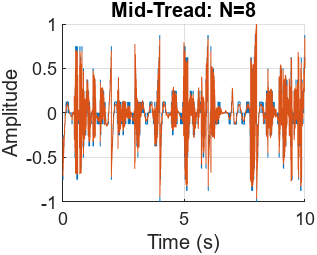
\includegraphics[width=.24\textwidth]{N8MT.png}\hfill
    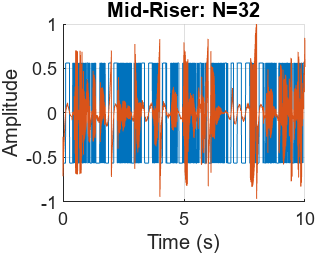
\includegraphics[width=.24\textwidth]{N32MR.png}\hfill
    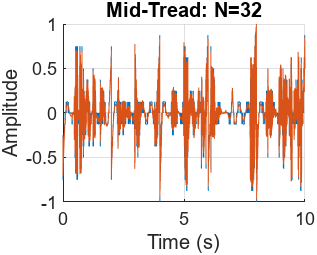
\includegraphics[width=.24\textwidth]{N32MT.png}\hfill
\end{figure}
\pagebreak
\end{document}